\begin{figure}[htbp]
\centering
\vspace{-2mm}
 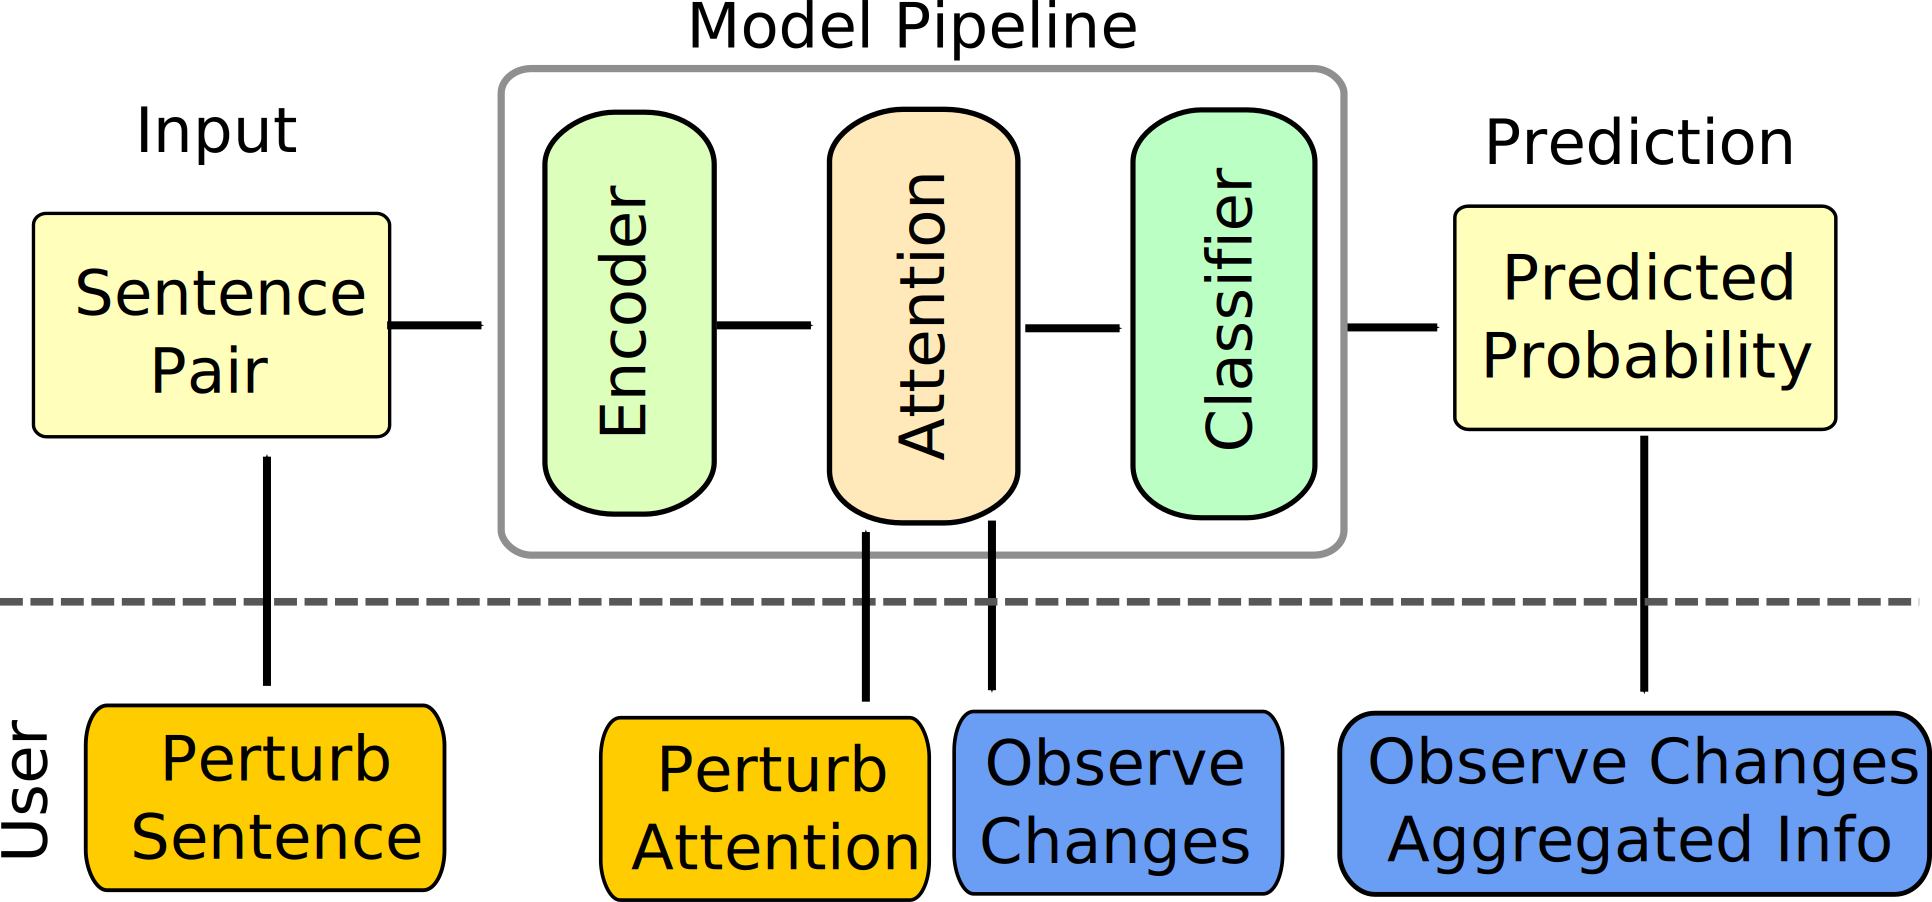
\includegraphics[width=1.0\linewidth]{pipeline}
 \caption{Language Inference Model Pipeline.}
\label{fig:modelPipeline}
\end{figure}

\section{The p-NLI System}
In this section, we describe the p-NLI system.

% Beside looking into the internal states, understanding how each of the component of the model interact with input and output as well as with each other is the crucial for truly examine the mechanism of the model.
%
Look at how the model work in action and interrogate relationship between different component, i.e., how the change made to one part of model affect the other pieces present, is the key to gain the full picture.
